% \documentclass[conference,10pt]{ieeeconf}
\documentclass[letterpaper, 10 pt, conference]{ieeeconf}
\IEEEoverridecommandlockouts
\overrideIEEEmargins
\usepackage{pstricks}
\usepackage{ifplatform}
\usepackage{xkeyval}
\usepackage{rotating}
\newtheorem{remark}{Remark}
\usepackage{graphics} % for pdf, bitmapped graphics files
% TEST-DEL: \usepackage[off]{auto-pst-pdf}
% \usepackage{mathptmx} % assumes new font selection scheme installed
\usepackage{times} % assumes new font selection scheme installed
\usepackage{amsmath} % assumes amsmath package installed
\usepackage{psfrag}
\usepackage{cancel}
\def\etal{\mbox{et al.}}
% \usepackage{pifont}
% \usepackage{flushend}
\usepackage[normalem]{ulem}
\usepackage{cite}
\usepackage{url}
\usepackage{color}
\input rgb
\def\blue#1{\textcolor{blue}{#1}}
\def\red#1{\textcolor{red}{#1}}
\def\orange#1{\textcolor{orange}{#1}}
\def\green#1{\textcolor{darkgreen}{#1}}
\usepackage{comment}
\usepackage{amssymb}
\usepackage{amsfonts}
%\usepackage[caption=false,font=footnotesize]{subfig}
\usepackage{subcaption}
% \usepackage{mathptmx}
%\usepackage{enumitem}
\usepackage{algorithmic}
\usepackage{algorithm}
\usepackage{pifont}% http://ctan.org/pkg/pifont
\newcommand{\cmark}{\ding{51}}%
\newcommand{\xmark}{\ding{55}}%
\newcommand{\smark}{$\bigstar$}%
\usepackage{booktabs}
%\input lamacro
\usepackage{lipsum}
\usepackage{array}
\newcolumntype{P}[1]{>{\centering\arraybackslash}p{#1}}
\newcommand{\JT}[1]{\textcolor{blue}{JT: #1}}
\newcommand{\AC}[1]{\textcolor{green}{AC: #1}}
\newcommand{\LP}[1]{\textcolor{red}{}}
\newcommand{\MN}[1]{\textcolor{orange}{MN: #1}}

\newcommand{\GR}[1]{\textcolor{magenta}{GR: #1}}
\newcommand{\assigned}[1]{\textcolor{purple}{Assigned To: #1}}
\newcommand{\budget}[1]{\textcolor{purple}{Page Budget: #1}}

\newcommand{\longonly}[1]{}
\newcommand{\shortonly}[1]{#1}

\newcommand{\maybeRemove}[1]{{\color{gray}#1}}
\newcommand{\xxx}{\textbf{\color{red}???}}
\newcommand{\LPafter}[1]{\longonly{\LP{#1}}}

% \renewcommand{\LP}[1]{}



\let\clipbox\relax
\usepackage{adjustbox}
%\usepackage{array}
\usepackage{booktabs}

\usepackage{CJKutf8}

\newcolumntype{R}[2]{%
    >{\adjustbox{angle=#1,lap=\width-(#2)}\bgroup}%
    l%
    <{\egroup}%
}
\newcommand*\rot{\multicolumn{1}{R{70}{1em}}}

\graphicspath{{figures/},{figures/new_diagrams/}}
\newcommand{\svgpath}{./images}

\usepackage{hyperref}
%\let\oldsection\section
%\renewcommand{\section}{\clearpage\oldsection}

%\allowdisplaybreaks[2]
\renewcommand{\baselinestretch}{0.97}
\textfloatsep = 6pt

% \let\subparagraph\relax
% \usepackage{titlesec}
% \usepackage[compact]{titlesec}
% \titlespacing{\section}{0pt}{2ex}{1ex}
% \titlespacing{\subsection}{0pt}{1ex}{0ex}
% \titlespacing{\subsubsection}{0pt}{0.5ex}{0ex}

\usepackage{mdwlist}
\let\stditemize\itemize
\let\endstditemize\enditemize
\let\itemize\undefined
\makecompactlist{itemize}{stditemize}

\let\stdenumerate\enumerate
\let\endstdenumerate\endenumerate
\let\enumerate\undefined
\makecompactlist{enumerate}{stdenumerate}

\setlength{\abovecaptionskip}{1pt}
\setlength{\belowcaptionskip}{1pt}

\usepackage[tracking=false,kerning=true,spacing=true]{microtype}
\pdfprotrudechars=2
\pdfadjustspacing=2

\makeatletter
\def\endthebibliography{%
  \def\@noitemerr{\@latex@warning{Empty `thebibliography' environment}}%
  \endlist
}
\makeatother

\title{\LARGE \bf
Duckieboat: 小型水上無人載具設計、開發與應用}

\author{Jui-Te Huang$^{1}$, Chao-Chun Hsu$^{1}$, and Sin-Kiat Lim$^{1}$}

\begin{document}
%\begin{CJK}{UTF8}{bsmi}
\begin{CJK}{UTF8}{bkai}

    \maketitle

    \thispagestyle{empty}
    \pagestyle{empty}

    %%%%%%%%%%%%%%%%%%%%%%%%%%%%%%%%%%%%%%%%%%%%%%%%%%%%%%%%%%%%%%%%%%%%%%%%%%%%%%%%

    \begin{abstract}

Duckieboat is an Unmanned maritime vehicle. Due to the cost of building an unmanned maritime vehicle is very expensive and time consuming. We decide to design a low-cost, high-durability, modular-design and easy-assemble boat which can implement in our research. It is also capable of transform into a variety of water applications, such as boat following, material supply, garbage collection and difficult environment marine exploration. We hope our Duckieboat will enhance the safety of sea in the future and can make the supply of water sports enthusiasts more convenient. Duckieboat also can implement in the teaching field, make students learn more about the related principles of autonomous boat.

Keywords: Unmanned System, Autonomous Navigation, Marine Robotics

\end{abstract}


    %%%%%%%%%%%%%%%%%%%%%%%%%%%%%%%%%%%%%%%%%%%%%%%%%%%%%%%%%%%%%%%%%%%%%%%%%%%%%%%%
    \section{Introduction}

Duckieboat is an Unmanned maritime vehicle. Due to the cost of building an unmanned maritime vehicle is very expensive and time consuming. We decide to design a low-cost, high-durability, modular-design and easy-assemble boat which can implement in our research. It is also capable of transform into a variety of water applications, such as boat following, material supply, garbage collection and difficult environment marine exploration. We hope our Duckieboat will enhance the safety of sea in the future and can make the supply of water sports enthusiasts more convenient. Duckieboat also can implement in the teaching field, make students learn more about the related principles of autonomous boat.

    \section{Hardware Structure}

\begin{figure}[h] % h means put this image here
	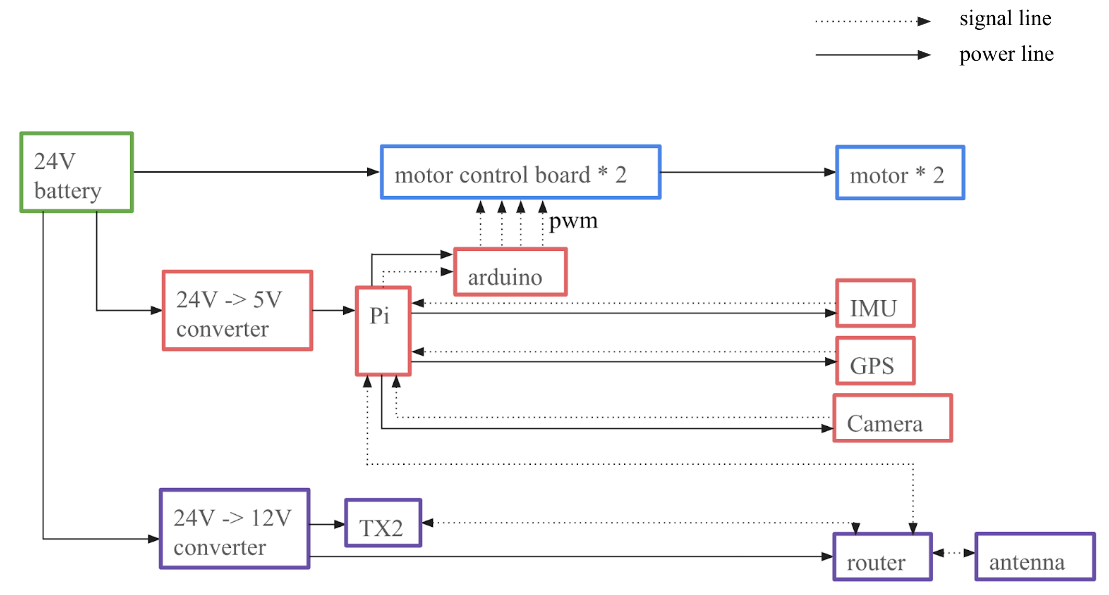
\includegraphics[width=0.8\columnwidth]{images/hardware.png}
	\centering
	\caption{signal and power flow}
	\label{figure:hardware}
\end{figure}

\subsection{Power Transmition}

For power transmission, this system needs 3 kinds of voltages, 24V, 5V, and 12V. 24V supply through two motor control boards then drive the two motors. 5V supply initially powered Raspberry pi, it will also supply Arduino UNO, IMU, GPS and pi camera with it’s USB ports. As to 12V, it will supply TX2 compute unit and router.

\subsection{Signal Transmition}

For signal transmission, Raspberry pi and TX2 will communicate through wifi, wifi router with an antenna will set on the boat. The Raspberry pi will collect the data from IMU, GPS and pi camera, after computing in Raspberry pi and image processing in TX2, it will send pwm signal (0~3.3V) to Arduino UNO, then Arduino will map the input signal from (0~3.3V) into (0~5V) to two motor control boards.

\subsection{hardware setting}
Most of the compute units and sensors mentioned above except two motors, GPS and antenna, will be placed in a waterproof box. There will have waterproof connectors while the wire needs to go out from the waterproof box.

\begin{figure}[h] % h means put this image here
	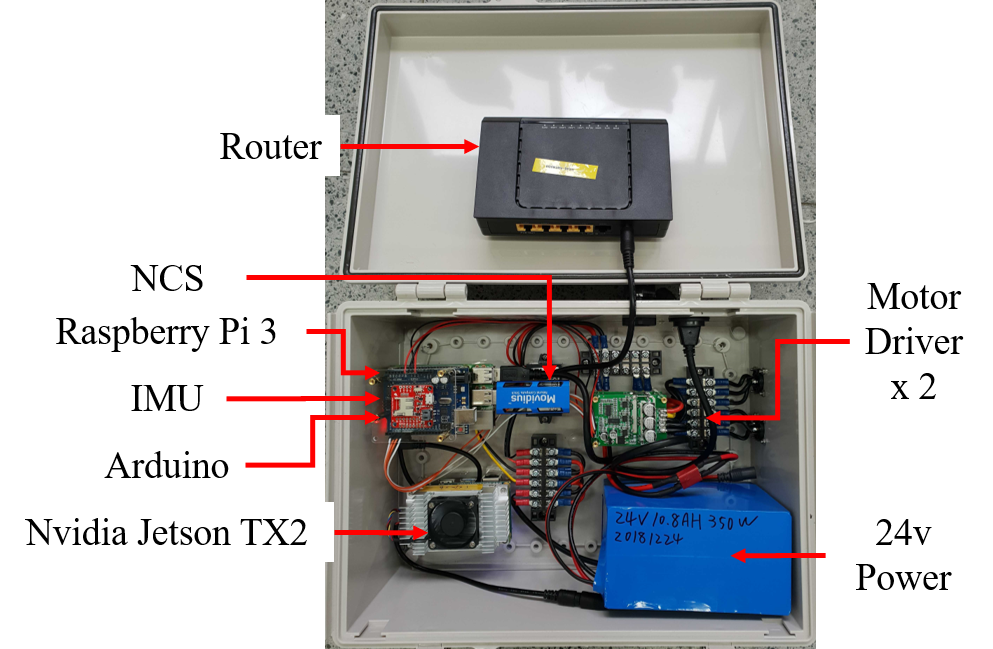
\includegraphics[width=0.8\columnwidth]{images/hardware_setting.png}
	\centering
	\caption{hardware setting}
	\label{figure:hardware_setting}
\end{figure}

\begin{figure}[h] % h means put this image here
	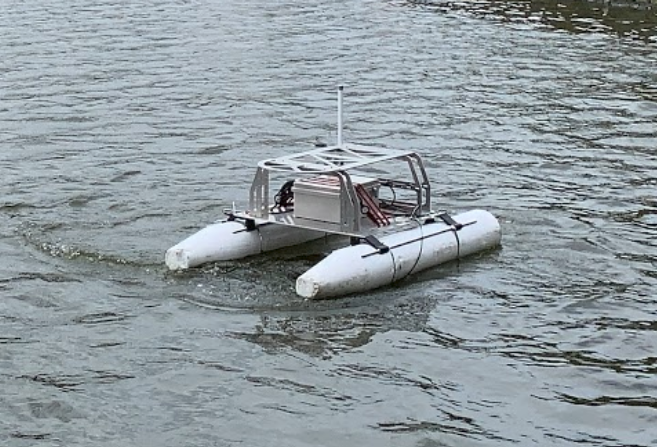
\includegraphics[width=0.8\columnwidth]{images/duckieboat.png}
	\centering
	\caption{The appearance of Duckieboat and where the waterproof box was placed.}
	\label{figure:duckieboat}
\end{figure}


    \section{Software Structure}

\subsection{Joystick Control}

We use ROS write a node to switch between autonomous motor command and user control motor command.

\subsection{Waipoint Navigation}

We use GPS and IMU data to create Odometry. And it is filtered by a kalman filter then we pass our odometry to the navigation node to creat the motor command.

\subsection{Track and Trail}

To track the object on the water surface. We use pi-camera to get the image ahead of the boat. Then pass this image to object detection node. Once detect the object. we pass the bounding box of the object to the tracking node. Finally create a motor command to the Joystick node.

\begin{figure}[h]
	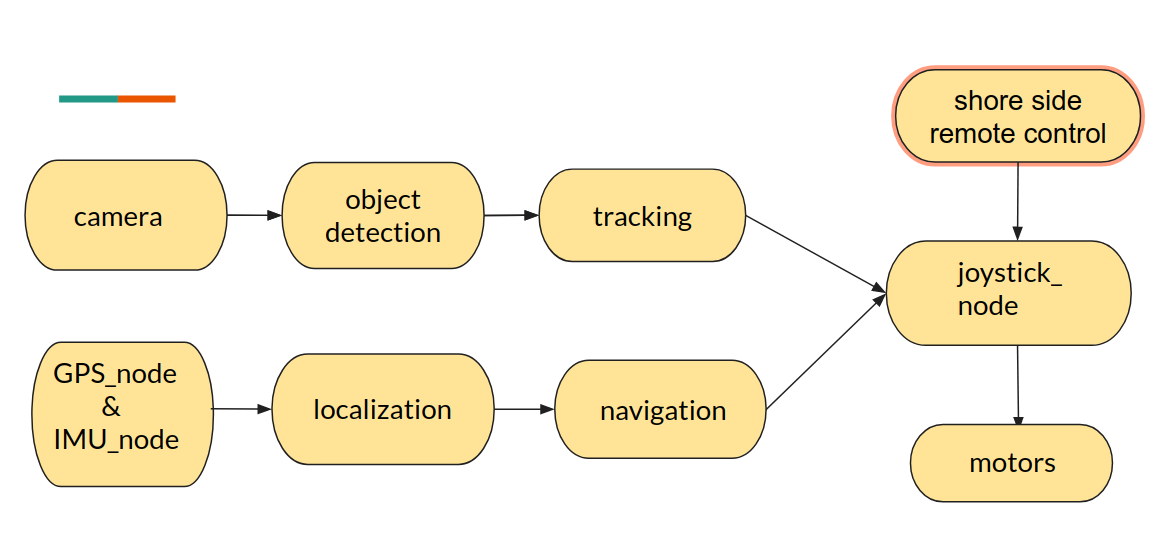
\includegraphics[width=1.0\columnwidth]{images/software_structure.png}
	\centering
	\caption{software structure}
	\label{figure:software_structure}
\end{figure}

    \section{Control Configuration}

\subsection{Differential Drive}

Using two motors will consume less power than using four motors and the cost also will be the lower-cost. But it cannot completely complete some of the more complicated moves, such as some seas have more reefs and avoid the boat hitting the rocks, so it needs precise movement.

\[LeftMotor = Y + X\]
\[RightMotor = Y-X\]
\begin{figure}[h]
	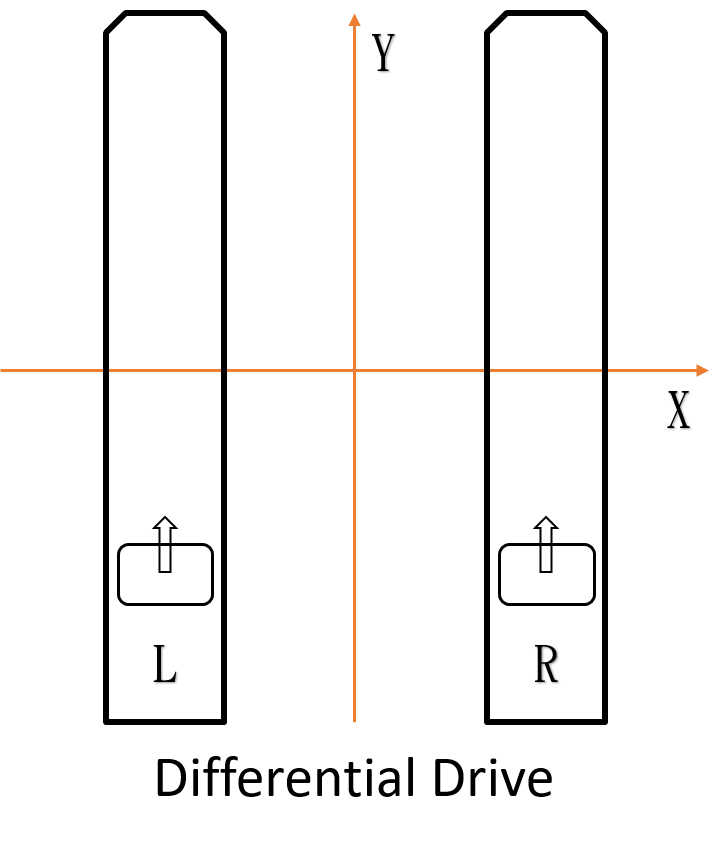
\includegraphics[width=0.5\columnwidth]{images/differential_drive.png}
	\centering
	\caption{differential drive motor config}
	\label{figure:differential_drive}
\end{figure}

\subsection{Omnidirectional Drive}

We choose to use four motors is because it can move omnidirectional, but it will consume more power and the motor is expensive will increase the cost of the Duckieboat. But it can move with precision, can be used in more complex environments.

\paragraph{Forward Kinematics}
\[Front Left Motor = Y + X + A \]
\[Front Right Motor = Y - X - A \]
\[Rear Left Motor = Y - X + A \]
\[Rear Right Motor = Y + X - A\]

\paragraph{Angle Control}

Get orientation of Yaw from IMU and go through the angle PID control to get angle(A). When get the angle(A) the Duckieboat will turn to the correct direction and stop the motor.

\begin{figure}[h]
	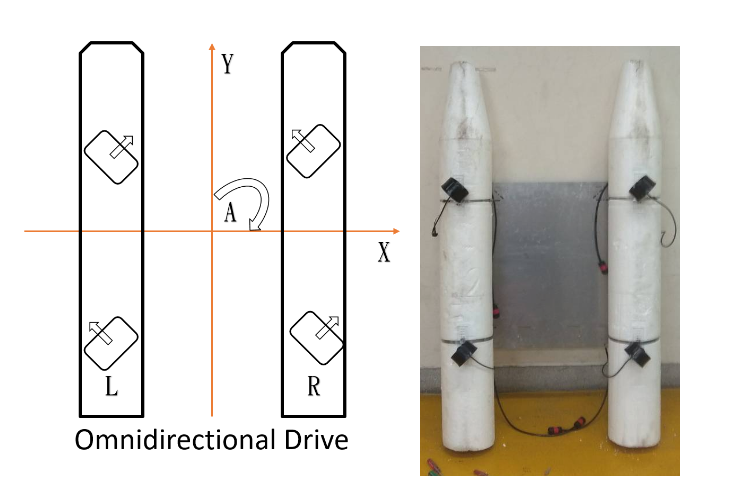
\includegraphics[width=1\columnwidth]{images/omni_drive.png}
	\centering
	\caption{omnidirectional drive motor config}
	\label{figure:omni_drive}
\end{figure}

\subsection{Conclusion}
We had already tried two different drive (Differential Drive and Omnidirectional Drive), the different drive can use in different environments, such as some areas have reefs and needs precise movement, we will prefer to use Omnidirectional Drive because we can avoid the boat hitting the rocks. Most of the time we will prefer to use Differential Drive because it consumes less power and more environmentally friendly.



    \section{Navigation}

Navigation is a basic task for Duckieboat, user can tap the destination on PC, while Duckieboat received data from PC through wifi, it will control it to where user demands.

\subsection{Localization}
We can get current position and orientation of Duckieboat from GPS and IMU. After we choose a destination(G), data output from both sensors will go through Kalman filter before entering the compute units. 

\subsection{Algorithm}
The distance(D) and angle(A) between boat and destination will be calculated, each result will go through a PID controller and send it to motor controllers to navigate Duckieboat to our desire destination.

\begin{figure}[h]
	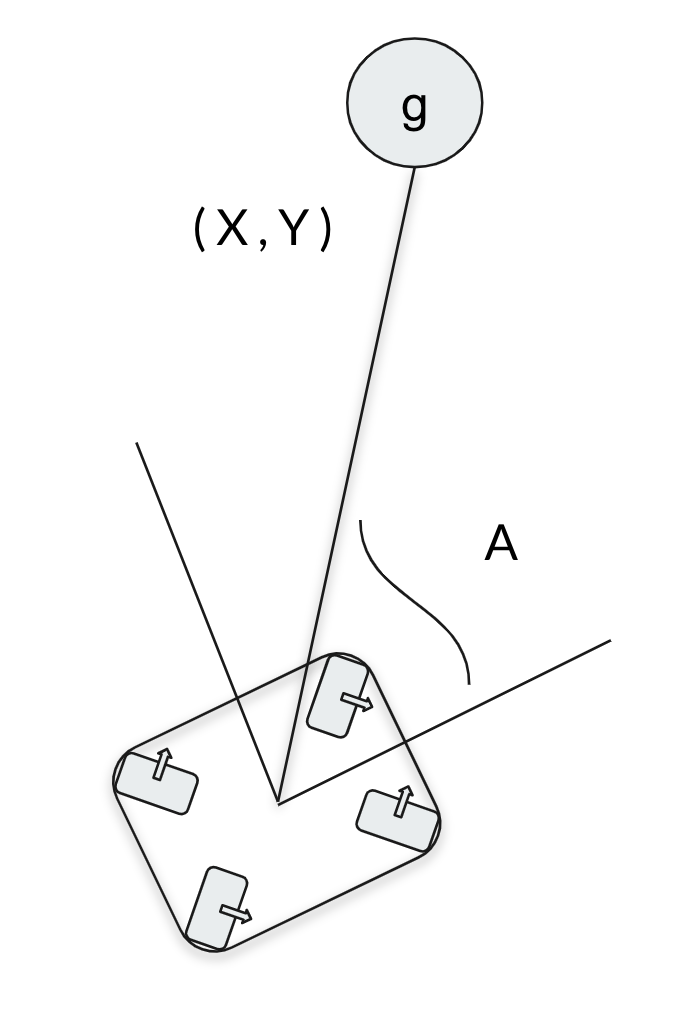
\includegraphics[width=0.5\columnwidth]{images/navigation.png}
	\centering
	\caption{navigation parameter}
	\label{figure:navigation}
\end{figure}

The frequency of data output from GPS and IMU is 10 Hz. Hence, we made Duckieboat enter station keeping mode after the distance is below 5 meters.



    \section{Object Detection}

\subsection{Model}

In order to track the kayaker. We must have an real time object detection model. So we choose MobileNet SSD to be our object detection model.
MobileNet separate the convolution process of traditional CNN models into depthwise convolution and pointwise convolution. Then combine the result later to achieve same effect of traditional convolution. But it can drastically reduce the computation.

\begin{figure}[h]
    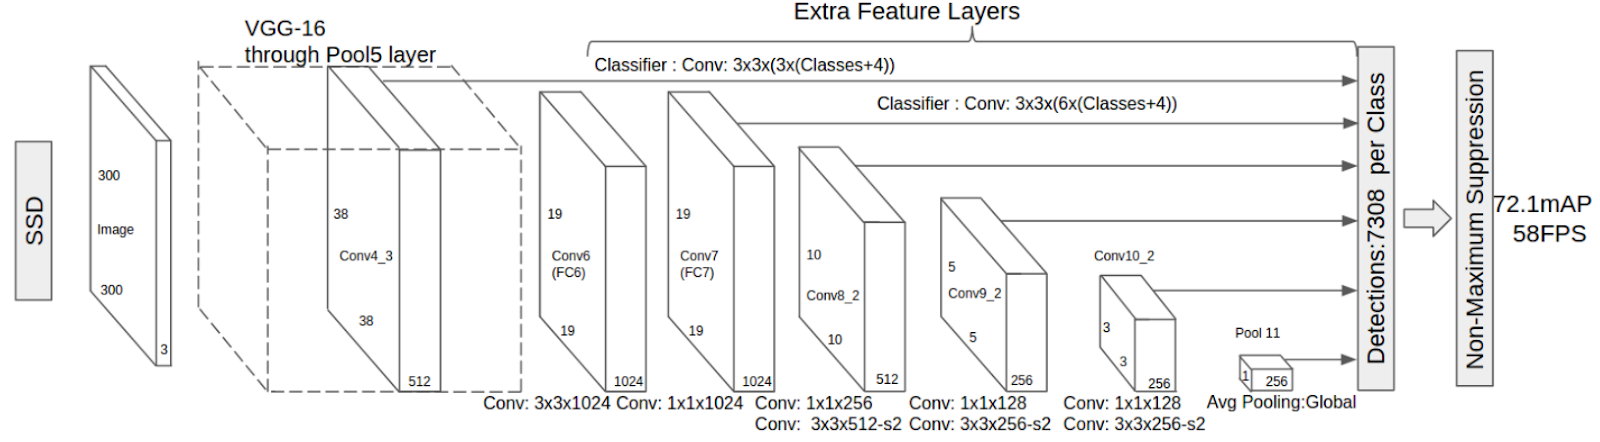
\includegraphics[width=1\columnwidth]{images/mobilenetssd.png}
    \centering
    \caption{SSD model}
    \label{figure:mobilenetssd}
\end{figure}

\subsection{Framework}

We use tensorflow object detection API to train the model. It has plenty of analysis tools for users to monitor training process. Once the model is trained. We use Nvidia jetson-TX2 to run the model. We can get up to 19 frames per second of detection. This is enough to implement kayaker tracking.

\subsection{Data collect and label}

We use 1951 photos of kayaker pictured by onboard picamera on the bamboo lake. Inorder to train a more generalized model. We also try to add 136 photos of kayaker downloaded on google photo. We use labelImg(https://github.com/tzutalin/labelImg) to label the bounding box of the Kayaker.

\begin{figure}[ht]
    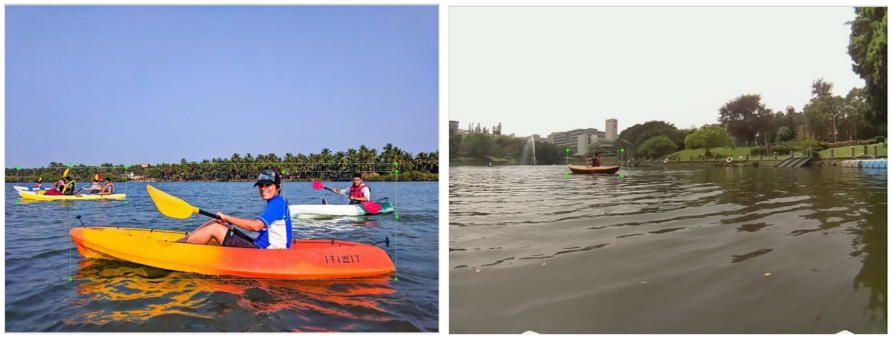
\includegraphics[width=1\columnwidth]{images/kayaker.png}
    \centering
    \caption{kayaker image data}
    \label{figure:kayaker}
\end{figure}

\subsection{Training}

We use GPU:RTX2070 trained for 52 minutes. With learning rate:$4e-3$, batch size:$24$, data split ratiao:$8/2$, epoch:$9265$

\begin{figure}[ht]
    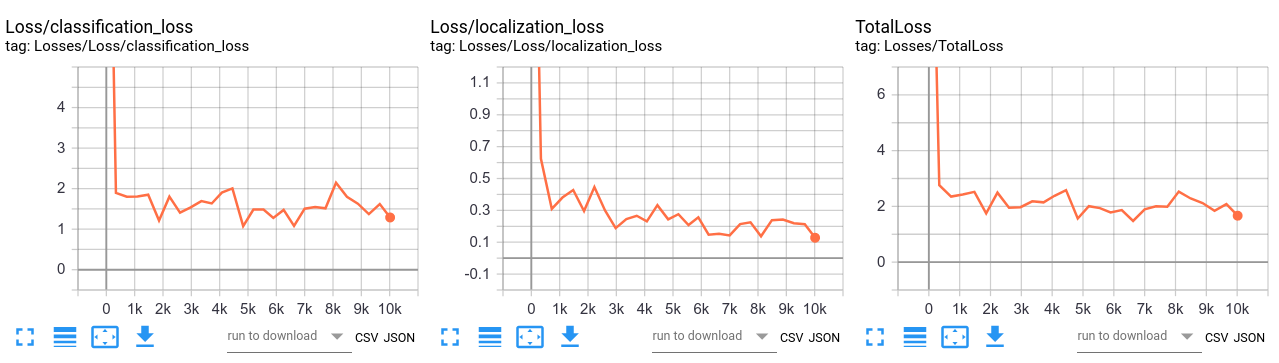
\includegraphics[width=1\columnwidth]{images/train_loss.png}
    \centering
    \caption{training loss}
    \label{figure:training_loss}
\end{figure}

\begin{figure}[ht]
    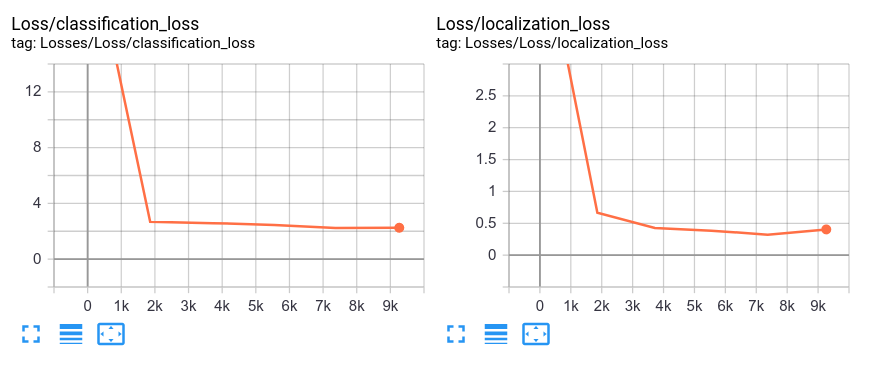
\includegraphics[width=1\columnwidth]{images/eval_loss.png}
    \centering
    \caption{evaluation loss}
    \label{figure:eval_loss}
\end{figure}

\subsection{Model analysis}

We use pr curve at iou=0.5 to analysis the model and compare the difference between pretrained model using COCO dataset boat class and our trained kayaker detection model. AP is improved from $77.09\%$ to $83.40\%$. 

\begin{figure}[ht]
    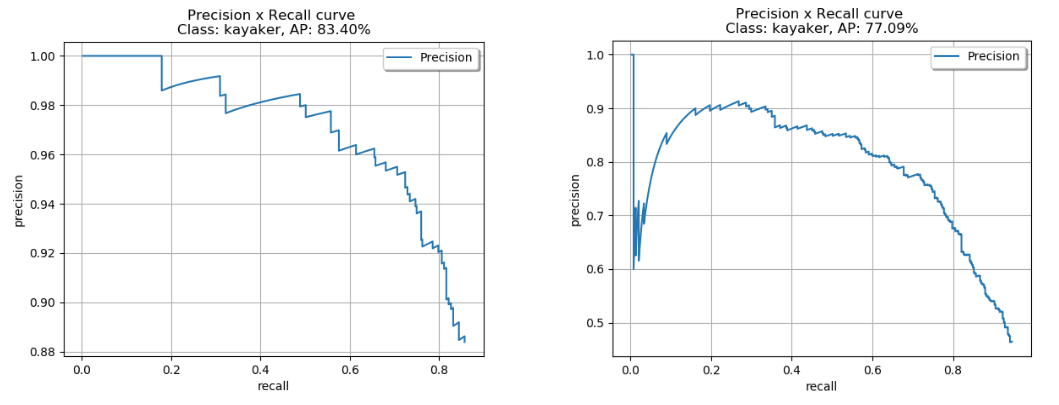
\includegraphics[width=1\columnwidth]{images/kayaker_pr.png}
    \centering
    \caption{left pic is pr curve of kayaker detection model, right pic is pretrained model}
    \label{figure:kayaker_pr}
\end{figure}
\begin{figure}[ht]
    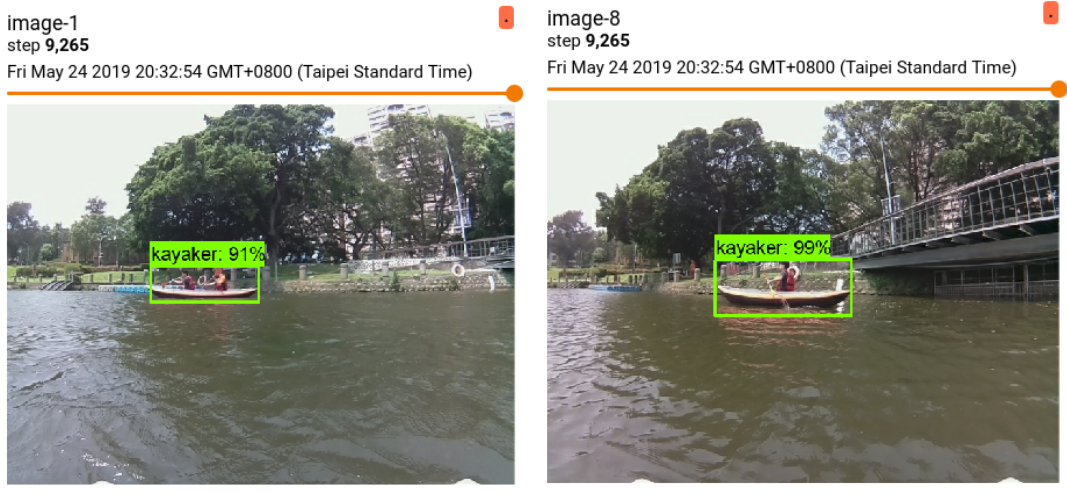
\includegraphics[width=1\columnwidth]{images/kayaker_dt.png}
    \centering
    \caption{detection result}
    \label{figure:kayaker_dt}
\end{figure}

\subsection{Trash detection}

We also try to detect the garbage floating on the water surface. for future applications like garbage collecting.but the challenge is the reflecting light of the water surface and the size of the bottle make it difficult to detect.

\begin{figure}[ht]
    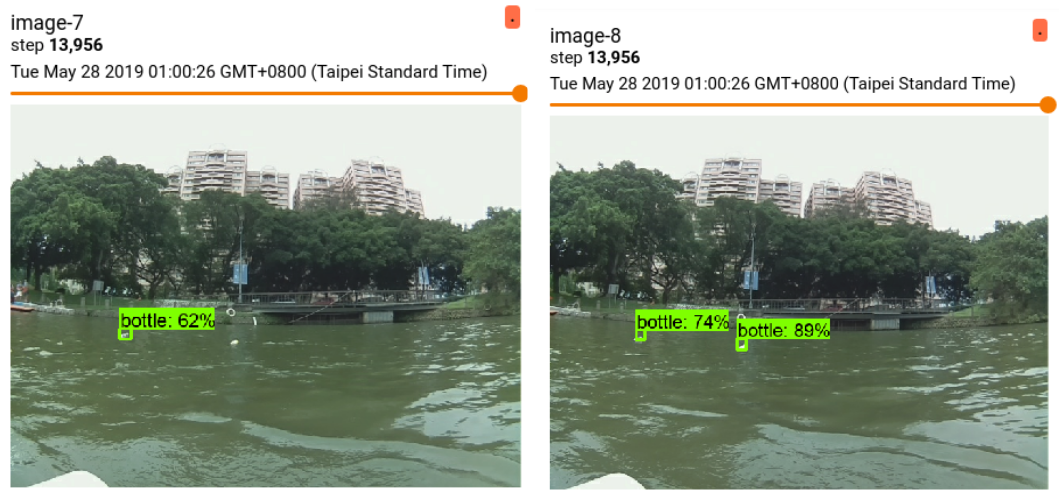
\includegraphics[width=1\columnwidth]{images/bottle.png}
    \centering
    \caption{bottle detection}
    \label{figure:bottle_dt}
\end{figure}


\begin{figure}[ht]
    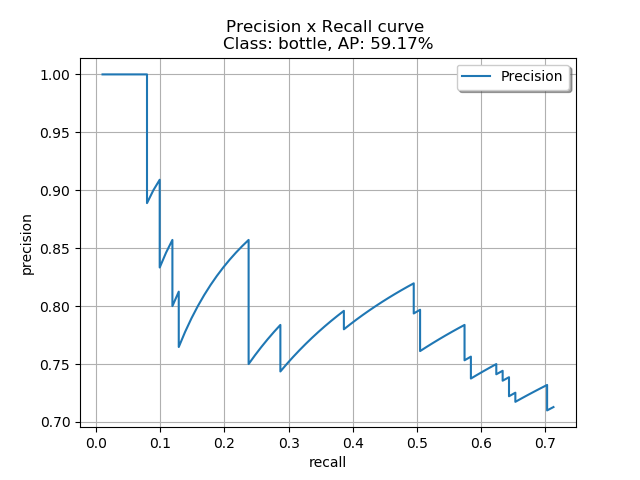
\includegraphics[width=1\columnwidth]{images/bottle_pr.png}
    \centering
    \caption{bottle detection pr curve}
    \label{figure:bottle_pr}
\end{figure}

    \section{Track and Trail}

\subsection{Bounding box tracking}

In order to keep track of the same bounding box we add an algorithm to give each bounding box an ID by comparing their position.

\begin{figure}[H]
    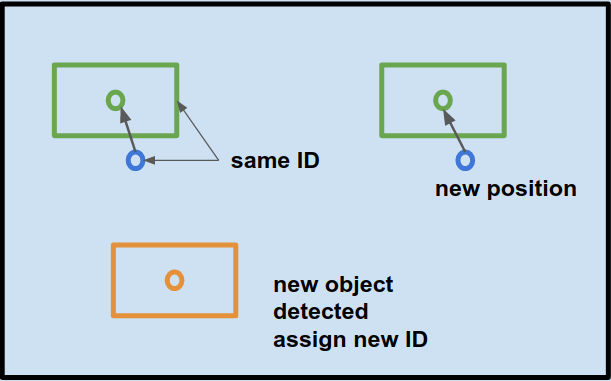
\includegraphics[width=1\columnwidth]{images/bbox.png}
    \centering
    \caption{bounding box id}
    \label{figure:bbox}
\end{figure}

\subsection{Tracking}

We use the bounding box of the target object as control signals. The height of the box indicate the distance between the target and boat. The position of the box indicates the orientation to the target. Then we use two PID controllers to control the distance and angle to keep track of the target.

\begin{figure}[H]
    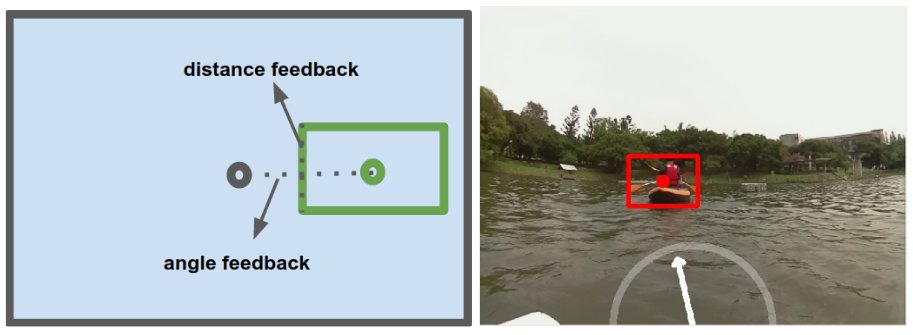
\includegraphics[width=1\columnwidth]{images/tracking.png}
    \centering
    \caption{tracking PID}
    \label{figure:tracking}
\end{figure}

    
    \section{Conclusion and Future Work}

\subsection{Conclusion}
Duckieboat is a low-cost, easy-assemble vehicle, it could widely implement to engineering education, maritime research and rescue missions.

\subsection{Future Work}
We plan to combine Duckieboat with the underwater unmanned maritime vehicle, looking forward to explore underwater environments, which is also unfamiliar to human.

We are also looking forward to upgrade our hardware to make it safer, durable and more user friendly.
\paragraph{}
enhance the communication between Duckieboat and shoreside.
\paragraph{}
build another communication type to seperate the command and joystick control.
\paragraph{}
change the material of the ski.
\paragraph{}
seperate the battery from the waterproof box.


    %\addtolength{\textheight}{-12cm} % This command serves to balance the column lengths
    % on the last page of the document manually. It shortens
    % the textheight of the last page by a suitable amount.
    % This command does not take effect until the next page
    % so it should come on the page before the last. Make
    % sure that you do not shorten the textheight too much.

    %%%%%%%%%%%%%%%%%%%%%%%%%%%%%%%%%%%%%%%%%%%%%%%%%%%%%%%%%%%%%%%%%%%%%%%%%%%%%%%%
    %\section*{APPENDIX}

    %Appendixes should appear before the acknowledgment.

    %This work was partially
    %supported by the National Science Foundation under grants IIS-1318392 and
    %IIS-1405259.

    %%%%%%%%%%%%%%%%%%%%%%%%%%%%%%%%%%%%%%%%%%%%%%%%%%%%%%%%%%%%%%%%%%%%%%%%%%%%%%%%

    \bibliographystyle{IEEEtran}
    \bibliography{arg-egbib}

\end{CJK}
\end{document}
